\begin{frame}{The Convergence Challenge in MCMC}
	\begin{itemize}
		\item \textbf{Ideal goal}: Assess whether MCMC chains have converged
		\item \textbf{Fundamental problem}:
		      \begin{itemize}
			      \item In general, impossible to know for sure that there is no problem
			      \item But we can sometimes know for sure that there \textit{is} a problem
		      \end{itemize}
		\item \textbf{Two phases of MCMC}:
		      \begin{itemize}
			      \item Transient phase (burn-in): mixing time
			      \item Stationary phase: Monte Carlo estimation
		      \end{itemize}
	\end{itemize}

	\vspace{0.5cm}
	\begin{center}
		\tikz{
			\draw[thick, ->] (0,0) -- (8,0) node[right] {Iterations};
			\draw[thick] (0,-0.1) -- (0,0.1);
			\draw[thick] (3,-0.1) -- (3,0.1);
			\draw[copenhagenred, ultra thick] (0,0.5) -- (3,0.5);
			\draw[blue, ultra thick] (3,0.5) -- (8,0.5);
			\node at (1.5, 1) {\color{copenhagenred} Burn-in};
			\node at (5.5, 1) {\color{blue} Sampling};
		}
	\end{center}
\end{frame}

\begin{frame}{Why Convergence Matters}
	\textbf{Non-converged chains:}
	\begin{itemize}
		\item Biased estimates
		\item Incorrect uncertainty quantification
		\item Missing important modes
		\item Unreliable inference
	\end{itemize}
\end{frame}

\begin{frame}{Motivating example}
	\begin{figure}
		\centering
		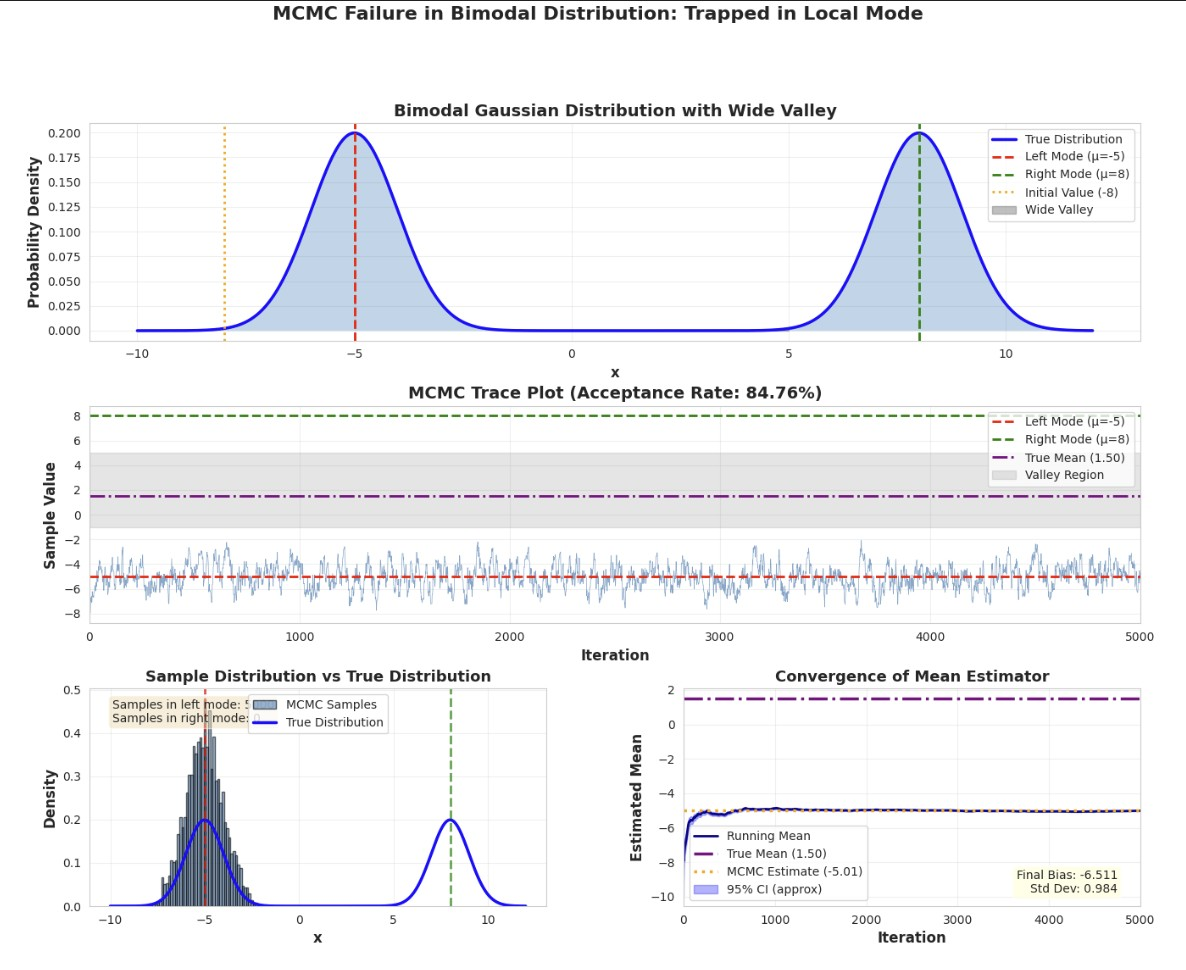
\includegraphics[width=0.6\textwidth]{bimodal.jpg}
		\caption{Trace plots of two MCMC chains that have not converged, illustrating the challenge of diagnosing convergence. Both chains appear stable but are sampling different regions of the parameter space.}
	\end{figure}
\end{frame}

\begin{frame}{The Intuition Behind Gelman-Rubin}
	\begin{block}{Core Idea}
		If MCMC chains have converged to the target distribution, then:
		\begin{itemize}
			\item Multiple chains started from different points should look similar
			\item Within-chain variance $\approx$ Between-chain variance 
		\end{itemize}
	\end{block}

	\textbf{Compare two sources of variance:}
	\begin{enumerate}
		\item \textcolor{blue}{Within-chain variance (W)}\\
		      How much each chain varies
		\item \textcolor{red}{Between-chain variance (B)}\\
		      How different chains are from each other
	\end{enumerate}
\end{frame}

\begin{frame}{Within-chain variance - $W$}
	Run $M$ chains. The sample mean of $M$ sample variances
	$$W  = \frac{1}{M} \sum_{m=1}^M \Big[\frac{1}{T-1} \sum_{t=1}^T (X_{m,t} - \bar{X}_m)^2\Big]$$
	We have that the expected sample variance for one chain is
	$$\mathbb{E}\Big[\frac{1}{T-1} \sum_{t=1}^T (X_{m,t} - \bar{X}_m)^2\Big] = \frac{T}{T-1} \Big(\sigma^2 - Var(\bar{X}_{m,.})\Big)$$
	making the estimator unbiased only in the case $Var(\bar{X}_{m,.}) = \sigma^2 / T$ (iid samples).

	For MCMC samples, $Var(\bar{X}_{m,.})$ is typically larger than $\sigma^2 / T$ due to
	autocorrelation, so $W$ underestimates $\sigma^2$.
\end{frame}

\begin{frame}{Between-chain variance - $B$}
	For the $M$ chains, we compute the variance of the chain means:
	$$B = \frac{1}{M-1} \sum_{m=1}^M (\bar{X}_{m,.} - \bar{X}_{..})^2$$
	where $\bar{X}_{..}$ is the mean across all chains. We have that
	$$\mathbb{E}[B] = Var(\bar{X}_{m,.})$$
\end{frame}

\begin{frame}{Estimators for Target Variance}
	We have 2 estimators for the target variance $\sigma^2$:

	$$W  = \frac{1}{M} \sum_{m=1}^M \Big[\frac{1}{T-1} \sum_{t=1}^T (X_{m,t} - \bar{X}_m)^2\Big]$$
	and
	$$V = \frac{T-1}{T}W + B = \Big(1-\frac{1}{T}\Big)W +B$$

	\vspace{0.3cm}
	$V$ weights the within-chain variance $W$ heavily when you have many samples, but
	adds between-chain variance $B$ to account for the fact that chains might not be
	fully mixed yet.

	\vspace{0.3cm}
	In case we start the chains from overdispersed initial values, we expect $B$ to be large,
	since chain means $\bar{X}_{m,.}$ are more spread out than they should be. Thus:
	$B$ overestimates $Var(\bar{X}_{m,.})$. This makes $V$ overestimate $\sigma^2$.
\end{frame}

\begin{frame}{The Gelman-Rubin Statistic}
	\begin{block}{Definition}
		$$\hat{R} = \sqrt{\frac{V}{W}}$$
	\end{block}

	\begin{columns}
		\column{0.4\textwidth}
		\begin{itemize}
			\item Original recommendation: $\hat{R} < 1.1$ for convergence.
			\item More recent advice: $\hat{R} < 1.01$ (Vehtari et al., 2021)
			\item But what does $\hat{R}$ really mean?
		\end{itemize}

		\column{0.6\textwidth}
		\begin{center}
			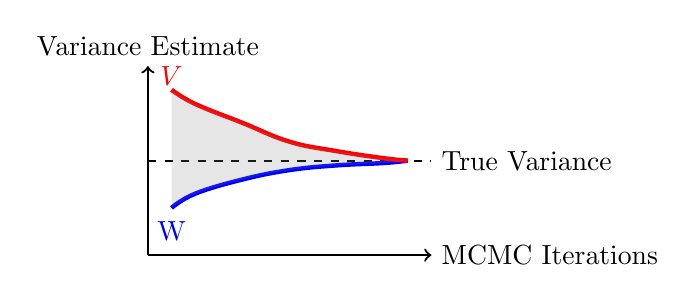
\begin{tikzpicture}[scale=0.6]
				% Draw variance evolution
				\draw[thick, ->] (0,0) -- (6,0) node[right] {MCMC Iterations};
				\draw[thick, ->] (0,0) -- (0,4) node[above] {Variance Estimate};

				% True variance line
				\draw[black, dashed, thick] (0,2) -- (6,2) node[right] {True Variance};

				% W line (underestimates initially)
				\draw[blue, ultra thick] plot[smooth, tension=0.7] coordinates
					{(0.5,1) (1,1.3) (2,1.6) (3,1.8) (4,1.9) (5,1.95) (5.5,2)};
				\node[blue] at (0.5,0.5) {W};

				% V line (overestimates initially)
				\draw[red, ultra thick] plot[smooth, tension=0.7] coordinates
					{(0.5,3.5) (1,3.2) (2,2.8) (3,2.4) (4,2.2) (5,2.05) (5.5,2)};
				\node[red] at (0.5,3.8) {$V$};

				% Shaded area
				\fill[gray, opacity=0.2] (0.5,1) -- plot[smooth, tension=0.7] coordinates
					{(0.5,1) (1,1.3) (2,1.6) (3,1.8) (4,1.9) (5,1.95) (5.5,2)}
				-- (5.5,2) -- plot[smooth, tension=0.7] coordinates
					{(5.5,2) (5,2.05) (4,2.2) (3,2.4) (2,2.8) (1,3.2) (0.5,3.5)} -- cycle;
			\end{tikzpicture}
		\end{center}

	\end{columns}
\end{frame}

\begin{frame}{Connection to Effective Sample Size}
	\begin{block}{Key Approximation (Vats \& Knudson, 2021)}
		$$\hat{R} \approx \sqrt{1 + \frac{M}{\text{ESS}}}$$
	\end{block}

	Where:
	\begin{itemize}
		\item $M$ = number of chains
		\item ESS = number of independent samples with the same standard error as a correlated sample.
	\end{itemize}

	\vspace{0.2cm}
	\textbf{Implications:}
	\begin{itemize}
		\item $\hat{R} = 1.1 \Rightarrow$ ESS $\approx 5M$ (5 independent samples per chain)
		\item $\hat{R} = 1.01 \Rightarrow$ ESS $\approx 50M$ (50 independent samples per chain)
	\end{itemize}

	\vspace{0.2cm}
	\begin{center}
		\color{copenhagenred} 5 effective samples per chain is too small for reliable inference!
	\end{center}
\end{frame}

\section{Limitations and Failure Modes}

\begin{frame}{Weaknesses of Gelman-Rubin}
	\begin{enumerate}
		\item \textbf{Only detects lack of convergence}
		\item \textbf{Cannot detect if all modes are found}
		      \begin{itemize}
			      \item Only checks if chains agree with each other
			      \item All chains might miss the same modes
		      \end{itemize}

		\item \textbf{Sensitive to initialization}
		      \begin{itemize}
			      \item Chains starting in the same wrong place
		      \end{itemize}
	\end{enumerate}
\end{frame}

\begin{frame}{Convergence Assessment}
	\begin{block}{Use Multiple Diagnostics}
		\begin{enumerate}
			\item \textbf{Gelman-Rubin statistic}: $\hat{R} < 1.01$
			\item \textbf{Effective Sample Size}
			\item \textbf{Trace plots}: Visual inspection
			\item \textbf{Autocorrelation}: Check mixing quality
		\end{enumerate}
	\end{block}

	\vspace{0.5cm}
	\textbf{Best Practices:}
	\begin{itemize}
		\item Use at least 4 chains (preferably more)
		\item Initialize chains from overdispersed starting points
		\item Run chains longer than you think necessary
	\end{itemize}
\end{frame}
